  This just says that, for each interval, we use the approximation that
  is most appropriate.  The function is continuous and
  once-differentiable everywhere, and is therefore well behaved for
  computational purposes.
  \begin{comment}
    In practice, in our problem the difference due to this refinement is displayed in Figure \ref{fig:IntExpFOCInvPesReaOpt45GapPlot}.
    \hypertarget{IntExpFOCInvPesReaOpt45GapPlot}{}
    \begin{figure}
      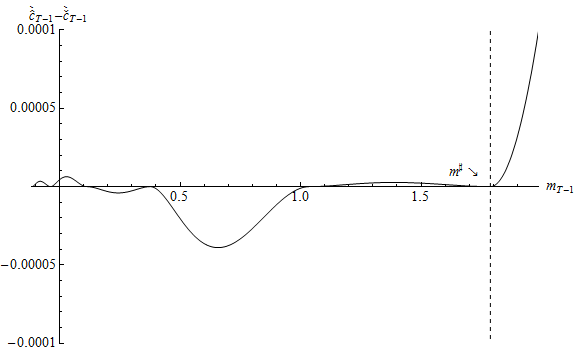
\includegraphics[width=6in]{./Figures/IntExpFOCInvPesReaOpt45GapPlot}
      \caption{Difference Between $\Alt{\Hi{\cFunc}}_{L, T-1}$ and $\Alt{\Hi{\cFunc}}_{H,T-1}$ is Small}
      \label{fig:IntExpFOCInvPesReaOpt45GapPlot}
    \end{figure}
  \end{comment}

  We now construct an upper-bound value function implied for a consumer whose spending behavior
  is consistent with the refined upper-bound consumption rule.

  For $\mNrm_{t} \geq \mNrm_{t}^{\#}$, this consumption rule is the same as before,
  so the constructed upper-bound value function is also the same.  However, for
  values $\mNrm_{t} < \mNrm_{t}^{\#}$ matters are slightly more complicated.

  Start with the fact that at the cusp point,
  \begin{equation*}\begin{gathered}\begin{aligned}
        \bar{\vFunc}_{t}(\mtCusp)  & = \uFunc(\bar{\cNrm}_{t}(\mtCusp))\mathbb{C}_{t}^{T} \\
        & =  \uFunc(\aboveMin \mtCusp  \MPCmax_{t})\mathbb{C}_{t}^{T}
        .
      \end{aligned}\end{gathered}\end{equation*}

  But for \textit{all} $\mNrm_{t}$,
  \begin{equation*}\begin{gathered}\begin{aligned}
        \bar{\vFunc}_{t}(\mNrm)  & = \uFunc(\bar{\cNrm}_{t}(\mNrm))+ \bar{\vEndStge}(\mNrm-\bar{\cNrm}_{t}(\mNrm)),
      \end{aligned}\end{gathered}\end{equation*}
  and we assume that for the consumer below the cusp point consumption is given by $\MPCmax \aboveMin \mNrm_{t}$ so for $\mNrm_{t}< \mtCusp$
  \begin{equation*}\begin{gathered}\begin{aligned}
        \bar{\vFunc}_{t}(\mNrm)  & = \uFunc( \MPCmax_{t} \aboveMin \mNrm)+ \bar{\vEndStge}((1-\MPCmax_{t})\aboveMin \mNrm),
      \end{aligned}\end{gathered}\end{equation*}
  which is easy to compute because $\bar{\vEndStge}(\aNrm_{t}) = \DiscFac \bar{\vFunc}_{t+1}(\aNrm_{t}\RNrm+1)$
  where $\bar{\vFunc}_{t}$ is as defined above because a consumer who ends the current period with assets exceeding
  the lower bound will not expect to be constrained next period.  (Recall again that we are merely constructing an object that is guaranteed to be an \textit{upper bound} for the value that the `realist' consumer will experience.)  At the gridpoints defined by the solution of the
  consumption problem can then construct
  \begin{equation*}\begin{gathered}\begin{aligned}
        \bar{\vInv}_{t}(\mNrm)  & = ((1-\CRRA)\bar{\vFunc}_{t}(\mNrm))^{1/(1-\CRRA)}
      \end{aligned}\end{gathered}\end{equation*}
  \MPCMatch{and its derivatives}{} which yields the appropriate vector for constructing $\check{\Chi}$ and $\check{\Koppa}$.  The rest of the procedure is analogous to that performed for the consumption rule and is thus omitted for brevity.

